%%%%%%%%%%%%%%%%%%%%%%%%%%%%%%%%%%%%%%%%%%%%%%%%%%%%%%%%%%%%%%%%%%%%%%%%%%%%%
%%%
%%% File: thesis.tex, version 1.9, May 2016
%%%
%%% =============================================
%%% This file contains a template that can be used with the package
%%% cs.sty and LaTeX2e to produce a thesis that meets the requirements
%%% of the Computer Science Department from the Technical University of Cluj-Napoca
%%%%%%%%%%%%%%%%%%%%%%%%%%%%%%%%%%%%%%%%%%%%%%%%%%%%%%%%%%%%%%%%%%%%%%%%%%%%%

\documentclass[12pt,a4paper,twoside]{report}         
\usepackage{cs}              
\usepackage{times}
\usepackage{graphicx}
\usepackage{latexsym}
\usepackage{amsmath,amsbsy}
\usepackage{amssymb}
\usepackage[matrix,arrow]{xy}
\usepackage[T1]{fontenc}
\usepackage{ae,aecompl}
%\usepackage{shortcut} %definitii pentru diacritice; 
\usepackage{amstext}
\usepackage{graphics}
\usepackage{ae,aecompl}
\usepackage{algorithm}
%\usepackage{algorithmic}
\usepackage{color}
\usepackage{enumitem}

% \mastersthesis
\diplomathesis
% \leftchapter
\centerchapter
% \rightchapter
\singlespace
% \oneandhalfspace
% \doublespace

\newcommand{\applicationTitle}{Land Drone}

\renewcommand{\thesisauthor}{Firstname LASTNAME}    %% Your name.
\renewcommand{\thesismonth}{June}     %% Your month of graduation.
\renewcommand{\thesisyear}{2018}      %% Your year of graduation.
\renewcommand{\thesistitle}{LICENSE THESIS TITLE} 
\renewcommand{\thesissupervisor}{scientific title Firstname LASTNAME}
\newcommand{\department}{\bf FACULTY OF AUTOMATION AND COMPUTER SCIENCE\\
COMPUTER SCIENCE DEPARTMENT}
\newcommand{\thesis}{LUCRARE DE LICEN'T'A}
\newcommand{\utcnlogo}{
\includegraphics[width=15cm]{img/tucn.jpg}}

\newcommand{\uline}[1]{\rule[0pt]{#1}{0.4pt}}
%\renewcommand{\thesisdedication}{P\u{a}rin\c{t}ilor mei}

\begin{document}
%\frontmatter
%\pagestyle{headings}

\newenvironment{definition}[1][Defini\c{t}ie.]{\begin{trivlist}
\item[\hskip \labelsep {\bfseries #1}]}{\end{trivlist}}



%\thesistitle                    %% Generate the title page.
%\authordeclarationpage                %% Generate the declaration page.

\pagenumbering{arabic}
\setcounter{page}{4}



\begin{center}
\utcnlogo

\department

\vspace{4cm}

{\bf \thesistitle} %LICENSE THESIS TITLE}

\vspace{1.5cm}

LICENSE THESIS

\vspace{6cm}

Graduate: {\bf Adrian BIRLADEANU}

Supervisor: {\bf \thesissupervisor}

\vspace{3cm}
{\bf \thesisyear}
\end{center}

\thispagestyle{empty}
\newpage

\begin{center}
\utcnlogo

\department

\end{center}
\vspace{0.5cm}

%\begin{small}
\begin{tabular}{p{7cm}p{8cm}}
 %\hspace{-1cm}& APPROVED,\\
 \hspace{-1cm}DEAN, & HEAD OF DEPARTMENT,\\
 \hspace{-1cm}{\bf Prof. dr. eng. Liviu MICLEA} & {\bf Prof. dr. eng. Rodica POTOLEA}\\  
\end{tabular}
 
\vspace{2cm}

\begin{center}
Graduate: {\bf \thesisauthor}

\vspace{1cm}

{\bf \thesistitle}
\end{center}

\vspace{1cm}

\begin{enumerate}
 \item {\bf Project proposal:} {\it Short description of the license thesis and initial data}
\item {\bf Project contents:} {\it (enumerate the main component parts) Presentation page, advisor's evaluation, title of chapter 1, title of chapter 2, ..., title of chapter n, bibliography, appendices.}
\item {\bf Place of documentation:} {\it Example}: Technical University of Cluj-Napoca, Computer Science Department
\item {\bf Consultants:}
\item {\bf Date of issue of the proposal:} November 1, 2016
\item {\bf Date of  delivery:} February 21, 2018 {\it (the date when the document is submitted)}
  \end{enumerate}
\vspace{1.2cm}

\hspace{6cm} Graduate: \uline{6cm} 

\vspace{0.5cm}
\hspace{6cm} Supervisor: \uline{6cm} 
%\end{small}

\thispagestyle{empty}


\newpage
$ $
%\begin{center}
%\utcnlogo

%\department
%\end{center}

\thispagestyle{empty}
\newpage

\begin{center}
\utcnlogo

\department
\end{center}

\vspace{0.5cm}

\begin{center}
{\bf
Declara\c{t}ie pe proprie r\u{a}spundere privind\\ 
autenticitatea lucr\u{a}rii de licen\c{t}\u{a}}
\end{center}
\vspace{1cm}



Subsemnatul(a) \\
\uline{14.8cm}, 
legitimat(\u{a}) cu \uline{4cm} seria \uline{3cm} nr. \uline{4cm}\\
CNP \uline{9cm}, autorul lucr\u{a}rii \uline{2.8cm}\\
\uline{16cm}\\
\uline{16cm}\\
elaborat\u{a} \^{\i}n vederea sus\c{t}inerii examenului de finalizare a studiilor de licen\c{t}\u{a} la Facultatea de Automatic\u{a} \c{s}i Calculatoare, Specializarea \uline{7cm} din cadrul Universit\u{a}\c{t}ii Tehnice din Cluj-Napoca, sesiunea \uline{4cm} a anului universitar \uline{3cm}, declar pe proprie r\u{a}spundere, c\u{a} aceast\u{a} lucrare este rezultatul propriei activit\u{a}\c{t}i intelectuale, pe baza cercet\u{a}rilor mele \c{s}i pe baza informa\c{t}iilor ob\c{t}inute din surse care au fost citate, \^{\i}n textul lucr\u{a}rii \c{s}i \^{\i}n bibliografie.

Declar, c\u{a} aceast\u{a} lucrare nu con\c{t}ine por\c{t}iuni plagiate, iar sursele bibliografice au fost folosite cu 
respectarea legisla\c{t}iei rom\^{a}ne \c{s}i a conven\c{t}iilor interna\c{t}ionale privind drepturile de autor.

Declar, de asemenea, c\u{a} aceast\u{a} lucrare nu a mai fost prezentat\u{a} \^{\i}n fa\c{t}a unei alte comisii de examen de licen\c{t}\u{a}.

\^{I}n cazul constat\u{a}rii ulterioare a unor declara\c{t}ii false, voi suporta sanc\c{t}iunile administrative, respectiv, \emph{anularea examenului de licen\c{t}\u{a}}.

\vspace{1.5cm}

Data \hspace{8cm} Nume, Prenume

\vspace{0.5cm}

\uline{3cm} \hspace{5cm} \uline{5cm}

\vspace{0.5cm}
\hspace{9.4cm}Semn\u{a}tura

\thispagestyle{empty}

\newpage


%\listoftables
%\listoffigures

%\clearpage 
%\newpage

%\begin{comment}
{\color{red}{\bf De citit \^{\i}nainte} (aceast\u{a} pagin\u{a} se va elimina din versiunea final\u{a})}:
\begin{enumerate}
 \item Cele trei pagini anterioare (foaie de cap\u{a}t, foaie sumar, declara\c{t}ie) se vor lista pe foi separate (nu fa\c{t}\u{a}-verso), fiind incluse \^{\i}n lucrarea listat\u{a}. 
 Foaia de sumar (a doua) necesit\u{a} semn\u{a}tura absolventului, respectiv a coordonatorului.
 Pe declara\c{t}ie se trece data c\^{a}nd se pred\u{a} lucrarea la secretarii de comisie.
 \item Pe foaia de cap\u{a}t, se va trece corect titulatura cadrului didactic \^{\i}ndrum\u{a}tor, \^{\i}n englez\u{a} (consulta\c{t}i pagina de unde a\c{t}i desc\u{a}rcat acest document pentru lista cadrelor didactice cu titulaturile lor).
 \item Documentul curent {\bf nu} a fost creat \^{\i}n MS Office. E posibil sa fie mici diferen\c{t}e de formatare. 
\item Cuprinsul \^{\i}ncepe pe pagina nou\u{a}, impar\u{a} (dac\u{a} se face listare fa\c{t}\u{a}-verso), prima pagin\u{a} din capitolul \emph{Introducere} tot a\c{s}a, fiind numerotat\u{a} cu 1. % Pentru actualizarea cuprinsului, click dreapta pe cuprins (zona cuprinsului va apare cu gri), Update field-$>$Update entire table.
\item E recomandat s\u{a} vizualiza\c{t}i acest document \c{s}i \^{\i}n timpul edit\u{a}rii lucr\u{a}rii. % după ce activaţi vizualizarea simbolurilor ascunse de formatare (apăsaţi simbolul  din Home/Paragraph).
\item Fiecare capitol \^{\i}ncepe pe pagin\u{a} nou\u{a}. % datorită simbolului ascuns Section Break (Next Page) care este deja introdus la capitolul precedent. Dacă ştergeţi din greşeală simbolul, se reintroduce (Page Layout -> Breaks).
\item Folosi\c{t}i stilurile predefinite (Headings, Figure, Table, Normal, etc.)
\item Marginile la pagini nu se modific\u{a}.
\item Respecta\c{t}i restul instruc\c{t}iunilor din fiecare capitol.
\end{enumerate}
 
%\end{comment}

\newpage

\tableofcontents
\newpage




%\subsection{Subsection}
%%Each table used in this document is labeled as Table x.y, where x represents the chapter number, and y shows the table number within the current chapter. Leave a blank line between and after each table, relative to the adjacent paragraphs (table~\ref{table:nonlin}).
%
%\begin{table}[ht]
%\caption{Nonlinear Model Results}
%\centering                          % tabel centrat
%\begin{tabular}{|c|c|c|c|}          % 4 coloane centrate
%\hline\hline                        % linie orizontala dubla
%Case & Method\#1 & Method\#2 & Method\#3 \\ [0.5ex]   % inserare tabel
%%heading
%\hline                              % linie orizontal simpla
%1 & 50 & 837 & 970 \\               % corpul tabelului
%2 & 47 & 877 & 230 \\
%3 & 31 & 25 & 415 \\[1ex]           % [1ex] adds vertical space
%\hline
%\end{tabular}
%  % titlul tabelului
%\label{table:nonlin}                % \label{table:nonlin} introduce eticheta folosita pentru referirea tabelului in text; referirea in text se va face cu \ref{table:nonlin}
%\end{table}
%
%Each figure used in the document must be cited within the text (ex: in figure x.y the system components are presented... ) and labeled. The labeling must be as Figure x.y where x represents the chapter number, and y shows the number of the figure within the current chapter.
% E.g.: figure \ref{fig:imag}.
%
%\begin{figure}[ht]
%    \centering
%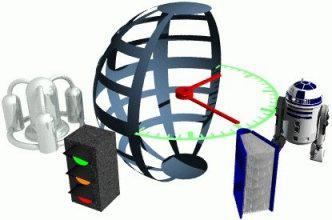
\includegraphics[]{img/test.jpg}
%    \caption{The figure`s name}
%    \label{fig:imag}
%\end{figure}
%
%Each chapter must start on a new page.

\usepackage{graphicx}


\chapter{Introduction - Project Context}
\label{ch:introduction}
\pagestyle{headings}

\section{Project context}
\label{sec:introduction-context}

\subsection{General Context}
\label{subsec:introduction-general-context}
With the increase of internet speed across the globe, possible among others to the appearance of 5G networks and, in
the near future, to the SpaceX Starlink network, it is now possible to stream increasingly larger data across the
internet. \
According to .., \ % todo: insert reference https://www.speedtest.net/global-index#mobile
the global mobile internet speed was of about 31Mbps for download and 11.88Mbps for upload. \
Although these values are still pretty low, they are bound to improve in the near future.
The highest values were achieved using 4G LTE and 4G LTE-A networks.

\begin{table}[ht]
    \caption{Average internet speed}
    \centering
    \begin{tabular}{|c|c|c|}
        \hline\hline
        Rank & Country & Download speed \[Mbps\] \\ [0.5ex]
        \hline
        1 & South Korea & 117.79 \\
        2 & Qatar & 77.07  \\
        3 & Norway & 72.80 \\
        4 & UAE & 69.72 \\
        5 & Australia & 68.87 \\
        6 & Canada & 67.57 \\
        7 & Netherlands & 62.86 \\
        8 & Croatia & 59.83 \\
        9 & China & 58.33 \\
        10 & Switzerland & 57.09 \\
        40 & Romania & 37.76
    \end{tabular}
    \label{table:internetSpeed}
\end{table}

% todo: mention ml/deep learning

\subsection{5G}
\label{subsec:5g}
According to ..\ % todo: quote https://www.telekom.com/en/company/details/5g-speed-is-data-transmission-in-real-time-544498
5G internet speeds should reach speeds of about 10Gbps, enough to stream video-audio in real time.
However, according to .. \ % todo: quote https://www.forbes.com/sites/bobodonnell/2019/11/22/real-world-5g-speeds/#3ec794804f96
and ..,\ % todo: quote https://5g.co.uk/guides/how-fast-is-5g/
such speeds cannot be reached with the current infrastructure, with download speeds averaging at about 130Mbps-240Mbps, \
with peaks at about 600Mbps.
However, certain variants have reached peaks of 1.8 Gbps (using mmWave 5G services) and event 1Tbps in controlled \
test environments.

It must be noted that these are only the early days of 5G networks, and that in the coming years these speeds are \
bound to improve.

According to .. \ % todo: quote https://web.archive.org/web/20190419231844/http://www.5gamericas.org/files/5115/4169/8314/5G_Americas_URLLLC_White_Paper_Final_11.8.pdf , https://en.wikipedia.org/wiki/5G
possible use cases for 5G networks include but are not limited to  Smart Factories (industrial control, robot control),\
 healthcare (remote diagnosis and surgery), entertainment (immersive entertainment, online gaming), transport \
industry (driver assistance, enhanced safety, autonomous driving, traffic management), energy sector (smart energy, \
smart grid).


\subsection{Satellite internet}
\label{subsec:satellite-internet}
As mentioned in .., \ % todo: quote https://www.forbes.com/sites/bobodonnell/2019/11/22/real-world-5g-speeds/#3ec794804f96
for 5G, the radio wave internet speed is inversely proportional to the distance covered. \
This means that regular 5G high speed internet will probably be limited to regions densely and medium populated and \
to research outposts because of infrastructure costs. \
A valid alternative for sparsely populated areas would be satellite internet. \
Several US companies have already begun taking steps towards a commercial solution. \
The most notable player is SpaceX with its project, Starlink, a network of several dozen thousands satellites in lower \
Earth orbit, in the range of 350\-550 km from Earth, as opposed to the average altitude of \
1000+ km for satellites in lower earth orbit. \
According to .. , % todo: quote https://www.pcmag.com/news/371511/spacexs-satellite-internet-plans-for-mid-2020-launch-in-the
the desired average speed is about 1Gbps. \
 .. % todo: quote https://spacenews.com/spacex-launches-second-batch-of-starlink-broadband-satellites/
mentions that tests with the US military achieved peak speeds of around 610 Mbps, while the network isn't fully \
functional yet, with thousands of satellites still to be sent to space. \
The official \href{https://www.starlink.com/}{Starlink} website it expects to reach coverage for northern US and \
Canada by 2020, and for the rest of the world by 2021.\
Other companies, including Amazon and OneWeb, have started work on deploying their own internet satellite network.

\subsection{Motivation}
\label{subsec:introduction-motivation}
With the rise of 5G internet and satellite-based internet, it will be increasingly easier to stream real-time data \
from one place in the world to another place on the opposite side. \
One use case for this increase in speed is the development of commercial drones controlled remotely over the internet.\
With 5G's speed, bandwidth and latency, it will be possible for a robot to transmit in virtually real-time audio-video \
data to a remote operator and to receive control commands from that operator.

\begin{figure}[ht]
    \label{fig:overview1}
    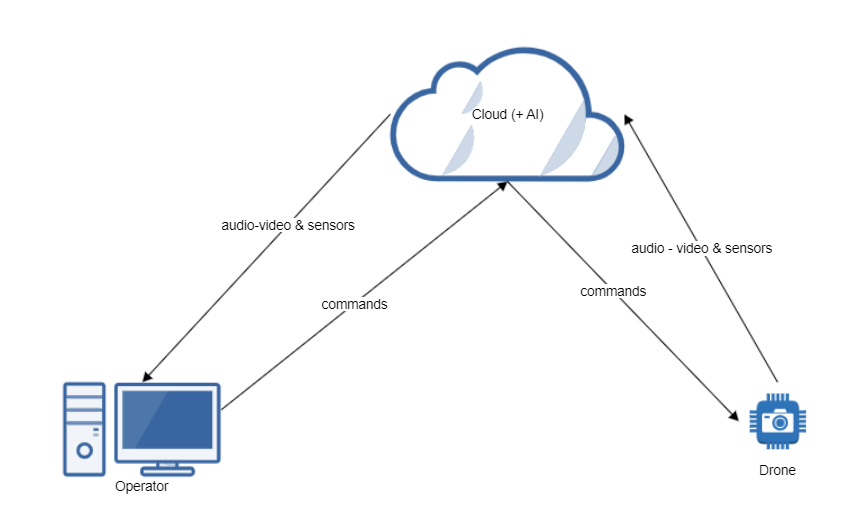
\includegraphics[width=15cm, height=10cm, keepaspectratio]{img/overview1.PNG}
    \caption{High Level Overview}
\end{figure}

This use case can be extended to autonomous robots. \
Instead of adding considerable computation capabilities to a robot (CPU, memory, GPU) os that it can run an AI, the \
robot could be fitted with minimal hardware designed only to transmit audio-video and receive commands from an AI that \
runs in the cloud. \
This way, if any malfunction occurs on the robot, the equipment could be easily replaced with lower costs because the \
equipment used was a lot cheaper than it would have been if hardware had to run the AI . \
Another option would be to use dedicated hardware that puts an emphasis on durability and can properly function in \
a wide range of conditions (rain, extreme low/high temperatures). \
Additionally, this type of setup would also use less energy in order to run, thus extending battery life and allowing \
higher autonomy.




%\usepackage{graphicx}


\chapter{Project Objectives and Specifications}
\label{ch:specification}

\section{Problem specification}
\label{sec:specification-specification}

Internet-controlled drones can take several forms and serve multiple purposes. \
This specific drone is a land drone (car) that streams video-only, not audio for now, and accepts \
commands from a web interface. \
Because 5G networks aren't accessible except via high-end smartphones, the robot will be connected \
to the internet via a 4G LTE mobile modem.

I have chosen a land drone because it is both easier and more affordable to build and test. \
However, most components (cloud server, web interface, drone - server communication) can be reused \
in order to build other types of drones (naval and flying drones).

Additionally, the drone will have person detection capabilities in order to \
meet certain security-related use cases, such as monitoring remote locations.

The current state-of-the-art in remote controlled drones is met on military drones. \
According to .. % todo: quote: https://www.forbes.com/sites/sebastienroblin/2019/09/30/dont-just-call-them-drones-a-laypersons-guide-to-military-unmanned-systems-on-air-land-and-sea/#76c957e62b00
the most popular control mechanisms are by radio and by satellite uplink. \
While the radio control requires a certain proximity of the drone to the operator (i.e., 100 miles), \
drones controlled via satellite uplink introduce a certain latency (image transmitted from a drone \
in Afghanistan may take up to 1.2 seconds to reach the operator in the US). \
High-Speed internet might provide a third control mechanism, that could remove the range limitation \
of the radio and decrease the latency of current satellite uplinks.

% todo: return here at home
Possible commercial use cases for this drone include wildlife observation,


\section{General Objectives}
\label{sec:specification-objectives}
The primary objective of this project is to create a drone that can be remotely controlled from \
half-way around the world.

\subsection{Use Cases}
\label{subsec:use-cases}
The project will need to meet the following use cases:

\subsubsection{\textbf{Login}}

\textbf{Primary Actor:} Drone Operator

\textbf{Stakeholders and Interests:}
\begin{enumerate}
    \item \textit{Drone Operator}: wants to be the sole person who controls \
            the drone at a given moment
    \item \textit{Drone owner}: wants to limit access to the drone video feed \
            and control to authorized personnel only
\end{enumerate}

\textbf{Postcondition:} The operator is granted access to the land drone

\textbf{Main Success Scenario}
\begin{enumerate}
    \item the operator goes to the drone url
    \item the operator inserts the username and password
    \item the cloud server validates the username and password
    \item the cloud server validates that no one else controls the drone
    \item the cloud server gives the operator access to the drone video \
            feed and controls
\end{enumerate}

\textbf{Extensions}
\begin{itemize}
    \item 3. The username or password is incorrect
        \begin{itemize}
            \item an error message is shown
            \item video feed and controls are disabled until the operator \
                    reloads the page
        \end{itemize}
    \item 4. Another operator already controls the drone
        \begin{itemize}
            \item the current operator is given access only to the video \
                    feed, while the first operator retains access to the controls
        \end{itemize}
\end{itemize}

\subsubsection{\textbf{View Drone Footage}}
\textbf{Primary Actor:} Drone Operator

\textbf{Stakeholders and Interests:}
\begin{enumerate}
    \item \textit{Drone Operator:} wants to view a live video feed from the drone
    \item \textit{Drone Operator and Owner} want to view the drone footage at a later date
\end{enumerate}

\textbf{Preconditions:} Drone operator has logged in and is the sole operator for the drone

\textbf{Main Success Scenario}
\begin{enumerate}
    \item Drone operator goes to the drone page
    \item Drone operator clicks on the \textbf{Start video feed} button
    \item The drone starts transmitting video feed
    \item The frontend shows the live video feed
\end{enumerate}

\textbf{Extensions}
\begin{itemize}
    \item The drone operator wants to save the video feed so that he can watch it at a later date
        \begin{itemize}
            \item After clicking on the \textbf{Start video feed} button, the operator clicks on the \
                    \textbf{Record feed} button
            \item The system starts recording the video feed
            \item The operator clicks on the \textbf{Stop recording} button
            \item The operator click on the \textbf{Download recording button}
            \item The system downloads the recording
        \end{itemize}
    \item The drone operator wants people to be highlighted
            \begin{itemize}
                \item After clicking on the \textbf{Start video feed}, but before clicking on the \
                        \textbf{Record feed} button, the operator presses on the \textbf{Highlight people} button
                \item The system shows the video feed, highlighting people and writing the names of the
                        known ones
            \end{itemize}
    \item A second operator wants to view the real time footage
            \begin{itemize}
                \item The second operator logs in
                \item The second operator views the same footage as the first
                \item The system disables all actions for the second operator (start recording, highlight people)
            \end{itemize}
\end{itemize}

\subsubsection{Control the drone}

\textbf{Primary Actor:} Drone Operator

\textbf{Stakeholders and Interests:}
\begin{enumerate}
    \item \textit{Drone operator} wants to move the drone in specific directions in order to meet his objectives
\end{enumerate}

\textbf{Preconditions:} Drone operator has logged in

\textbf{Main Success Scenario}
\begin{enumerate}
    \item The drone operator starts video feed and waits for it
    \item The drone operator controls the drone using the keyboard arrow keys
\end{enumerate}

\textbf{Extensions}
\begin{itemize}
    \item A second operator enters the drone page while the first operator control the drone
            \begin{itemize}
                \item The system disables the controls for the second operator
            \end{itemize}
\end{itemize}

% todo: go here
The presented use cases can be applied in the following fields:
\begin{enumerate}
    \item \textbf{Wildlife observation} the robot can be used to observe wild animals from a distance in areas with \
        decent internet coverage (minimum 7.2Mbps upload speed) % todo: maybe update value
    \item \textbf{Perimeter patrol} the robot can be used to patrol remote open areas where it's not possible to \
        mount security cameras (forests, borders)
\end{enumerate}


\section{Functional Requirements}
\label{sec:functional-requirements}

In software engineering, a functional requirement is a function of a system or its components. \
Such a function consists of a specific set of inputs, a behavior and an output. \
Functional requirements describe what the system \
is expected to do in order to accomplish its purpose and reach the desired results.

The functional requirements I have set out to achieve are mostly based on the use cases presented above. \
They are the following:
\begin{enumerate}
    \item live video feed from the drone to a web interface
    \item full control of the drone from a web interface
    \item recording capabilities for the live video feed
    \item option to highlight people
    \item limit of one active operator, with multiple passive operators having access to just the video feed, not the commands
\end{enumerate}

\section{Non-Functional Requirements}
\label{sec:non-functional-requirements}

In software engineering, a non-functional requirement refers to a system's quality characteristics and attributes, \
unlike functional requirements which refer to a system's functions. \
Non-functional requirements are used to \
evaluate all operations of the system, not just a specific component or behavior. \
They can be split into 2 \
categories: execution requirements (like security, performance) and evolution requirements (like scalability,
testability, extensibility). \
In the following subsections we will present in detail all the non-functional requirements.

\subsection{Performance}
\label{subsec:specification-performance}
Performance is one of the most important requirements of the system and is measured in several possible ways:
\begin{itemize}
    \item Video latency
    \item Video FPS
    \item Response time to commands
\end{itemize}

The video latency is measured in milliseconds since the image displayed was taken. \
Since the project won't be using 5G internet networks, but 4G LTE, I set out to achieve an average of \
15FPS with a latency of 500ms and a command response time of 100ms.

\subsection{Deployment}
\label{subsec:deployment}
The deployment will consist of hardware deployment (the drone itself plus its configuration) and software \
deployment (the control UI and other proxy and processing servers). \
The first step is the software deployment, which will be done in a kubernetes cluster. \
This can be done with relative ease. \
THe second step is the drone deployment, which includes a step for configuring the drone (writing the \
ip address to which video feed will be sent and the ip address from which commands will be received).

\subsection{Scalability and extendability}
\label{subsec:specification-scalability}
Scalability of the system refers to the ease with each the system can accommodate an increased \
number of users and data from distributors without changing the core of the application. \
On the one hand, the  application is centered on a single drone, with several possible operators. \
On the other hand, the application will be deployed in a Kubernetes cluster, meaning a new instance can easily \
be deployed for more drones.

Extendability refers to the ease with which new functional requirements can be accommodate as \
the number of users and their expectations increase.
One obvious direction of extending is adding more transmission mediums.
The current drone is designed to communicate using 4G LTE networks.
However, users may want to control the drone via Bluetooth or radio waves.
Therefore, the drone should be designed to easily accommodate these requirements.

\subsection{Usability}
\label{subsec:specification-usability}
Usability is the capacity of a system to allow its users to perform their \
tasks safely, effectively and efficiently, all the while offering an \
enjoyable experience.

In this project I aim to make the robot easy to control from any larger \
terminal (tablet, laptop or PC) without imposing certain hardware requirements \
from user devices (like having a state-of-the-art GPU).

\subsection{Security}
\label{subsec:specification-security}
% todo: complete security
to be completed

\chapter{Bibliographic research}
\label{ch:research}

% https://www.ericsson.com/en/reports-and-papers/white-papers/drones-and-networks-ensuring-safe-and-secure-operations
% https://web.stanford.edu/class/cs231a/prev_projects_2016/deep-drone-object__2_.pdf

\section{Remote Drone Control}
\label{sec:research-remote-drone-control}
The article ~\cite{ericsson1} also approaches the topic of drone control. \
According ot it, most current drone use cases cover the situation in which the drone \
operator is in line of sight of the drone and has full control over it, with autonomous \
drones operating outside line of sight gaining more and more importance today. \
However, in the future the most common drone use cases will be the ones in which the drone \
operates autonomously outside line of sight ir without supervision.

\begin{figure}[ht]
    \label{fig:drone-uses}
    %\centering
    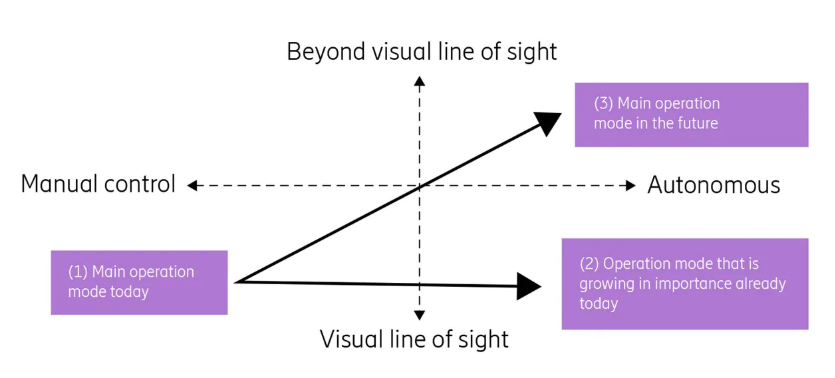
\includegraphics[width=15cm, height=50cm,keepaspectratio]{img/drone_uses.png}
    \caption{Drone Uses according to ~\cite{ericsson1}}
\end{figure}

In ~\cite{ericsson1} the author mentions three different options for drone communication and control:
\begin{enumerate}
    \item \textbf{satellite technology} is currently in use today for some drones; \
            its drawbacks include high latency and costs and low throughput
    \item \textbf{dedicated drone terrestrial network} its drawbacks also include high \
            costs and the time it would take to setup an adequate coverage for drones
    \item \textbf{existing terrestrial mobile networks} they have low latency and costs and \
            high throughput; \
            additionally, they have also proven to be secure and robust
\end{enumerate}

Additionally, other requirements can be accomplished using 4G LTE and 5G features. \
For instance, drone tracking can be implemented using the mobile positioning service and \
could be queried from the mobile network.

Drone control is also mentioned in ~\cite{forbes1} . \
The article also mentions 2 possible control methods that are actively used and that \
partially overlap over those mentioned above. \
These are:
\begin{enumerate}
    \item \textbf{radio waves} these have limited range (an example of 100 miles is given);
    \item \textbf{satellite uplink} it takes footage an average 1.2-second delay to go from \
            a drone in Afghanistan to the operator in Virginia
\end{enumerate}

~\cite{forbes1} also does a classification of drones according to how they are commanded. \
Three classes of drones emerge:
\begin{enumerate}
    \item \textbf{remotely piloted} an operator has full control, while the drone can do \
            minimal actions by its own, like avoid crashing
    \item \textbf{semi-autonomous} the drone can perform all or some missions without any \
            human interaction, however an operator exists that can take over control at \
            any time
    \item \textbf{fully autonomous} the drone is engineered to accomplish its mission \
            without any human interaction or supervision; \
            the command link can be missing
\end{enumerate}

\section{Object Detection}
\label{sec:research-object-detection}
In recent years, convolutional neural networks have been used more and more in \
the field of object detection. \
According to ~\cite{deepLearning}, A convolutional neural network (CNN) is a \
subclass of multilayer neural networks in which at least one layer applies \
a convolution on its input data instead of matrix multiplication.\
CNNs have seen a rise in use in object detection since 2012, when \
a CNN developed by ~\cite{imagenet} won the ImageNet Large Scale Visual \
Recognition Challenge for the first time. \
The CNN managed to reduce the top-1 (actual label differs from predicted label) \
 and top-5 (actual label is not in the predicted top 5 most likely labels) \
error rates from 47.1\% respectively 28.2\% to 37.5\% respectively 17\%. \
Additionally, the authors mentioned that the performance was limited by the \
existing hardware and dataset
Ever since, the contest has been won by convolutional neural networks. \
By 2016, the top-5 error rate dropped to 3.6\%.

% todo: mention SSD vs YOLO


In the paper~\cite{deepDrone}, the authors also attempt to create a drone capable \
of detecting people, with a few differences:
\begin{itemize}
    \item the drone is an airborne one
    \item image processing is done on the drone itself
\end{itemize}

The authors designed an algorithm to detect and track a single person at a time.
They used a Faster RCNN neural network to detect a person.
Once the drone detected an object, it stopped applying the neural network on \
new images.
Instead, it applied a KCF tracking algorithm as longs as the object was still in \
the image.
Once the KCF algorithm detected that he object was no longer in the image, \
the drone stopped applying the tracking algorithm and switched back to the \
detection neural network.
The authors also experimented with a YOLO detector, but they found that although it is \
faster than Faster RCNN, it is less accurate, especially when it comes to small and \
remote people.

The authors tested the tracking and detection algorithms on multiple GPUs, with the \
results shown in th table below:

\begin{table}[ht]
    \caption{Detection and Tracking Results}
    \centering
    \begin{tabular}{|c|c|c|c|}
        \hline\hline
        Hardware Platform & GTX 980 & TX1 & TK1 \\
        \hline
        Power & 150W & 10W & 7W \\
        Detection & 0.17s & 0.6s & 1.6s \\
        Tracking & 5.5ms & 14ms & 14ms \\
        \hline
    \end{tabular}
    \label{table:deep-drone-results}
\end{table}

Since the image processing is done on the drone itself, the power consumption of \
the CPU and GPU must also be taken into consideration in order to determine the \
autonomy of the drone.

\section{Object Tracking}
\label{sec:research-tracking}
%todo: add introduction
In ~\cite{OpencvTracking}, the author present a status of the most \
popular tracking algorithms from opencv.
After analysing multiple algorithms (CSRT, KCF, Boosting, MIL, TLD, \
MedianFlow, MOSSE, GOTURN), the author comes to the following \
conclusions:
\begin{itemize}
    \item \textbf{CSRT} should be used when higher tracking accuracy \
            is required and the program can tolerate a smaller throughput
    \item \textbf{KCF} should be used when the program requires greater \
            throughput and faster FPS at the expense of a slightly \
            lower accuracy
    \item \textbf{MOSSE} should be used when the speed is of absolute \
            importance
\end{itemize}

In ~\cite{OpencvTracking2} the author also compares the different \
tracking algorithms, adding the FPS for each algorithm.
The KCF tracker reached 409 FPS, but it failed to recover from full \
object occlusion.
The MOSSE tracker reached an astounding 2671 FPS, but it lacked \
behind deep learning based trackers in performance.
Even more, the author mentions that the algorithm looses precision \
even for objects in normal movement.
As for CSRT, it gives higher accuracy, but it reached only 32 FPS.


%Bibliographic research has as an objective the establishment of the references for the \
%project, within the project domain/thematic. While writing this chapter (in general the \
%whole document), the author will consider the knowledge accumulated from several \
%dedicated disciplines in the second semester, 4$^{th}$ year (Project Elaboration \
%Methodology, etc.), and other disciplines that are relevant to the project theme.
%
%Represents about 15\% of the paper.
%
%Each reference must be cited within the document text, see example below (depending \
%on the project theme, the presentation of a method/application can vary).
%
%
%This section includes citations for conferences or workshop~\cite{BellucciLZ04}, \
%journals~\cite{AntoniouSBDB07},
%and books~\cite{russell1995artificial}.
%
%In paper~\cite{AntoniouSBDB07} the authors present a detection system for moving obstacles based on stereovision and ego motion estimation.
%The method is ... {\it discus the algorithms, data structures, functionality, specific aspects related to the project theme, etc.}... Discussion: {\it pros and cons}.
%
%In chapter~\ref{ch:analysis} of~\cite{strunk}, the {\it similar-to-my-project-theme algorithm} is presented, with the following features ...
%
%
%\section{Title}
%\section{Other title}



\chapter{Analysis and Theoretical Foundation}
\label{ch:analysis}

%Together with the next chapter takes about 60\% of the whole paper
%
%The purpose of this chapter is to explain the operating principles of the implemented application.
%Here you write about your solution from a theory standpoint - i.e. you explain it and you demonstrate its theoretical properties/value, e.g.:
%\begin{itemize}
% \item used or proposed algorithms
% \item used protocols
% \item abstract models
% \item logic explanations/arguments concerning the chosen solution
% \item logic and functional structure of the application, etc.
%\end{itemize}
%
%{\color{red} YOU DO NOT write about implementation.
%
%YOU DO NOT copy/paste info on technologies from various sources and others alike, which do not pertain to your project.
%}

\section{Overview}
\label{sec:analysis-overview}
The project consists of several geographically-distributed components communicating \
to each other.
Since we are talking about a remote-controlled robot, it is obvious that 2 \
of these components are the robot and the control interface.
An important factor in determining what the other components are is the \
type of communication between the robot and the control interface (how the \
robot will transmit the video and how the controller will transmit the \
commands): Peer-to-peer or client-server.

In a client-server architecture, both the controller and the robot are connected \
to a server, and the server is in charge of relaying control commands from controller \
to the robot, and of processing robot images and transmitting them further to the \
controller.
In this architecture, image processing is only done once server-side, after which \
the result can be sent to multiple clients.
However, the server must make sure  only one controller client can send control \
messages to the robot.
This entails two more components: an image processor (that is in charge of processing \
robot images) and one server that is in charge of sending robot images to clients and \
of sending client commands to the robot.

The other type of architecture is Peer-to-peer.
In this case, the robot sends the video directly to the controllers, thus eliminating \
some communication overhead.
However, this introduces a new issue related to image processing.
If the image processing is done on the robot, then the robot will most likely require \
a GPU in order to speed up the processing and allow real-time video transmission.
However, this leads to a higher energy consumption and lower autonomy.
On the other hand, if the image processing is done on the machines on which the controller \
runs, then that machine will require a powerful GPU, which contradicts our usability \
requirements, which states that the users controlling the robot should be albe to use any \
larger screen, no matter the hardware.
Additionally, the robot should be aware of all controllers so that it known where \
to transmit the images, which introduces more coupling between the robot and \
controller.

Having considered the arguments above, I decided to go with the client-server \
architecture.
Besides the fact that it allows running object detection on specialized hardware \
without impacting the drone autonomy or requiring state-of-the-art GPU for controllers,\
it also decouples the drone from controllers.

\begin{figure}[ht]
    \label{fig:high-level-arch}
    %\centering
    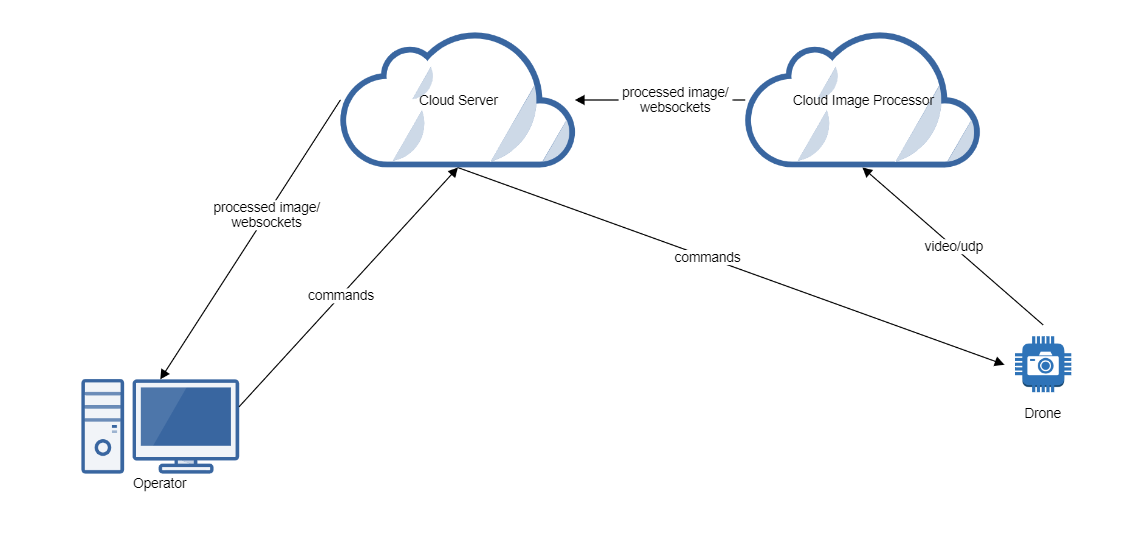
\includegraphics[width=15cm, height=50cm,keepaspectratio]{img/overview.png}
    \caption{High Level Architecture}
\end{figure}

Once I decided upon the architecture, I had to decide what type of \
client I would implement.
There were three possible options:
\begin{enumerate}
    \item Desktop client
    \item Mobile client
    \item Browser client
\end{enumerate}

After carefully considering all three options, I decided to implement \
a browser client for the following reasons:
\begin{enumerate}
    \item \textbf{Cross-platform support} Browser clients run on all \
            modern browsers on all desktop and mobile platforms.
            A Desktop application would have to have at least  3 \
            distributions (Linux, Windows, MacOS), while a mobile \
            platform would need to have at least 2 distributions
            (IOS and Android)
    \item \textbf{Application Update} Since the web client's source \
            reside on the server and are downloaded every time a user \
            runs the application, I have full control over what \
            version runs on the users' machines and don't have to \
            rely on them to update their applications or maintain \
            deprecated APIs in production so that older versions of \
            clients can still run.
    \item \textbf{Versatility} There is a possibility that future \
            requirements might be incompatible \
            with a browser application.
            With that in mind, there are open-source technologies \
            that can turn browser applications \
            into native desktop or native mobile applications.
\end{enumerate}




\section{Communication Protocols}
\label{sec:analysis-comms-protocols}
As seen in the diagram ~\ref{fig:high-level-arch},
every image is transmitted twice: once from drone to the server, and once from \
the server to the controller.
Ideally, in order to reduce latency, we would use UDP sockets for both transmissions.
However, since the controller should work in a browser, the connection between the controller \
and the server should be TCP.
As for the transmission between robot and the server, we are free to use UDP sockets, \
even if this means some packets could be dropped.
However, since the transmission will be done on Google premium quality networks, \
packet loss is expected to be low to zero.
As a result, the transmission between server and controller is expected to be slower \
than the transmission between robot and server (since TCP sockets require several round-trips \
in order to validate the content and possibly retransmit packets).
In order to minimize the effects of the TCP connections, the server should be \
geographically located as close as possible to the controller.
The closest datacenters to Romania are in Frankfurt and Milan for Amazon and in \
Frankfurt and Zurich for Google, with a Warsaw datacenter in construction.

As for the drone commands, these cannot be lost, so they will be transmitted using \
TCP sockets.
The most efficient TCP method of communication between a browser based \
application and a server is using websockets, which will be presented \
below.

\subsection{Websockets}
\label{subsec:analysis-websockets}
According to ~\cite{TeamTreeHouseWebSockets}, websockets appeared \
due to the need to establish efficient bi-directional connections \
between browser applications and servers.
After 2005, when AJAX appeared, which allowed browser applications \
to query a server for data without reloading the web page, \
developers became more interested in establishing bi-directional \
communication between client and server.
The first method was using long-polling.
As defined by ~\cite{WikiLongPolling}, long polling is a technique \
in which the client executes a normal connection, but expects that \
the server could not respond in a short while.
The server keeps the connection open up until it has new information \
that it can transmit as an HTTP/S response.
Then the client closes the existing HTTP/S request and makes a \
new one.
The downside of long polling is that both the initial HTTP/S \
request and the response contains a lot of specific HTTP headers \
and cookies, most or all of which are useless.
This introduces a considerable latency, especially when the number \
of concurrent connection grows.

Websockets appeared as a way to minimize latency, allowing true \
bi-directional communication.
Websockets are initialized with an HTTP request to the server, \
though there are a few differences.
The http/s scheme is replaced with an ws/s scheme specific to \
websockets.
Additionally, the request also contains an \textit{Upgrade} \
headers with the value \textit{websocket}

\begin{verbatim}
GET ws://localhost:8080/ HTTP/1.1
Origin: http://localhost:8080
Connection: Upgrade
Host: localhost:8080
Upgrade: websocket
\end{verbatim}

If the server has support for websockets, it sends back a response \
that also contains the \textit{Upgrade} header.

\begin{verbatim}
HTTP/1.1 101 WebSocket Protocol Handshake
Date: Wed, 17 Jun 2020 10:07:34 GMT
Connection: Upgrade
Upgrade: WebSocket
\end{verbatim}

After this handshake completes, the server and client replace the \
HTTP connection with a websocket connection which uses the same \
TCP/IP connection.
Then both the server and the client can send data to each other \
in a truly bi-directional communication.
The data is transmitted as websockets messages, each message \
consisting of multiple frames.
Only after all the frames have been received can the receiver \
begin to process the data.

Even though frames still require an additional 4\-12 frames \
of data in order for them to be routed correctly, the \
overhead is still considerably smaller than the overhead for \
normal HTTP requests, and the latency is reduced considerably.


\section{Algorithms}
\label{sec:analysis-algorithms}

\subsection{Object detection}
\label{subsec:analysis-object-detection}

For object detection I have chosen to use deep neural networks due to their \
increased performance (speed and accuracy) compared to other ML-based algorithms.\
More specifically, I decided to use the  MobileNetV2~\cite{mobilenet2} neural \
network with SSD (single shot detection).
MobileNet works as a feature extractor, with the output of its last layers \
connected to the input of the SSD network.

In order for deep neural networks to be effective, they need to be trained on \
large datasets. \
Some common such datasets are:
\begin{itemize}
    \item the Microsoft COCO dataset ~\cite{COCO} (about 300k images, out of \
            which more than 200k are labeled)
    \item the KITTI dataset ~\cite{kitti}
    \item Open Images dataset ~\cite{openimages} (over 1.7 million images)
\end{itemize}

A neural network takes a considerable amount of time to train on such datasets \
even with state-of-the-art hardware. \
For this reason, there are a number of pre-trained models available on the \
internet.
\footnote{https://github.com/tensorflow/models/blob/master/research/object\_detection/g3doc/detection\_model\_zoo.md} \
contains a list of pre-trained models that could be used for object detection.
The most efficient, taking into consideraiton both accuracy and execution \
speed, seems to be \textbf{ssdlite\_mobilenet\_v2\_coco}, which is why I \
chose to use it the drone.

\subsection{Object Tracking}
\label{subsec:analysis-object-tracking}
I also considered using tracking algorithms in conjunction \
with detection algorithms.
However, after careful analysis, I decided that the performance \
impact brought by the tracking algorithms would be too great \
compared to the business value.
On the one hand, detection algorithms should be run every frame \
in order to detect possible new objects.
If I applied tracking algorithms as well, in most cases the \
bounding boxes generated by the tracker and by the detector \
would overlap or share \~80\% surface, in which case the most \
likely case would be that the tracking algorithm would need \
correction.


\section{Robot}
\label{sec:analysis-robot-control}
In order to meet all functional requirements, the robot must consist of \
a central processing unit, a chassis, 4 dc motors and wheels, a motor shield, \
a camera and a 4G adapter, as shown in figure ~\ref{fig:robot-scheme}.

\begin{figure}[ht]
    \label{fig:robot-scheme}
    %\centering
    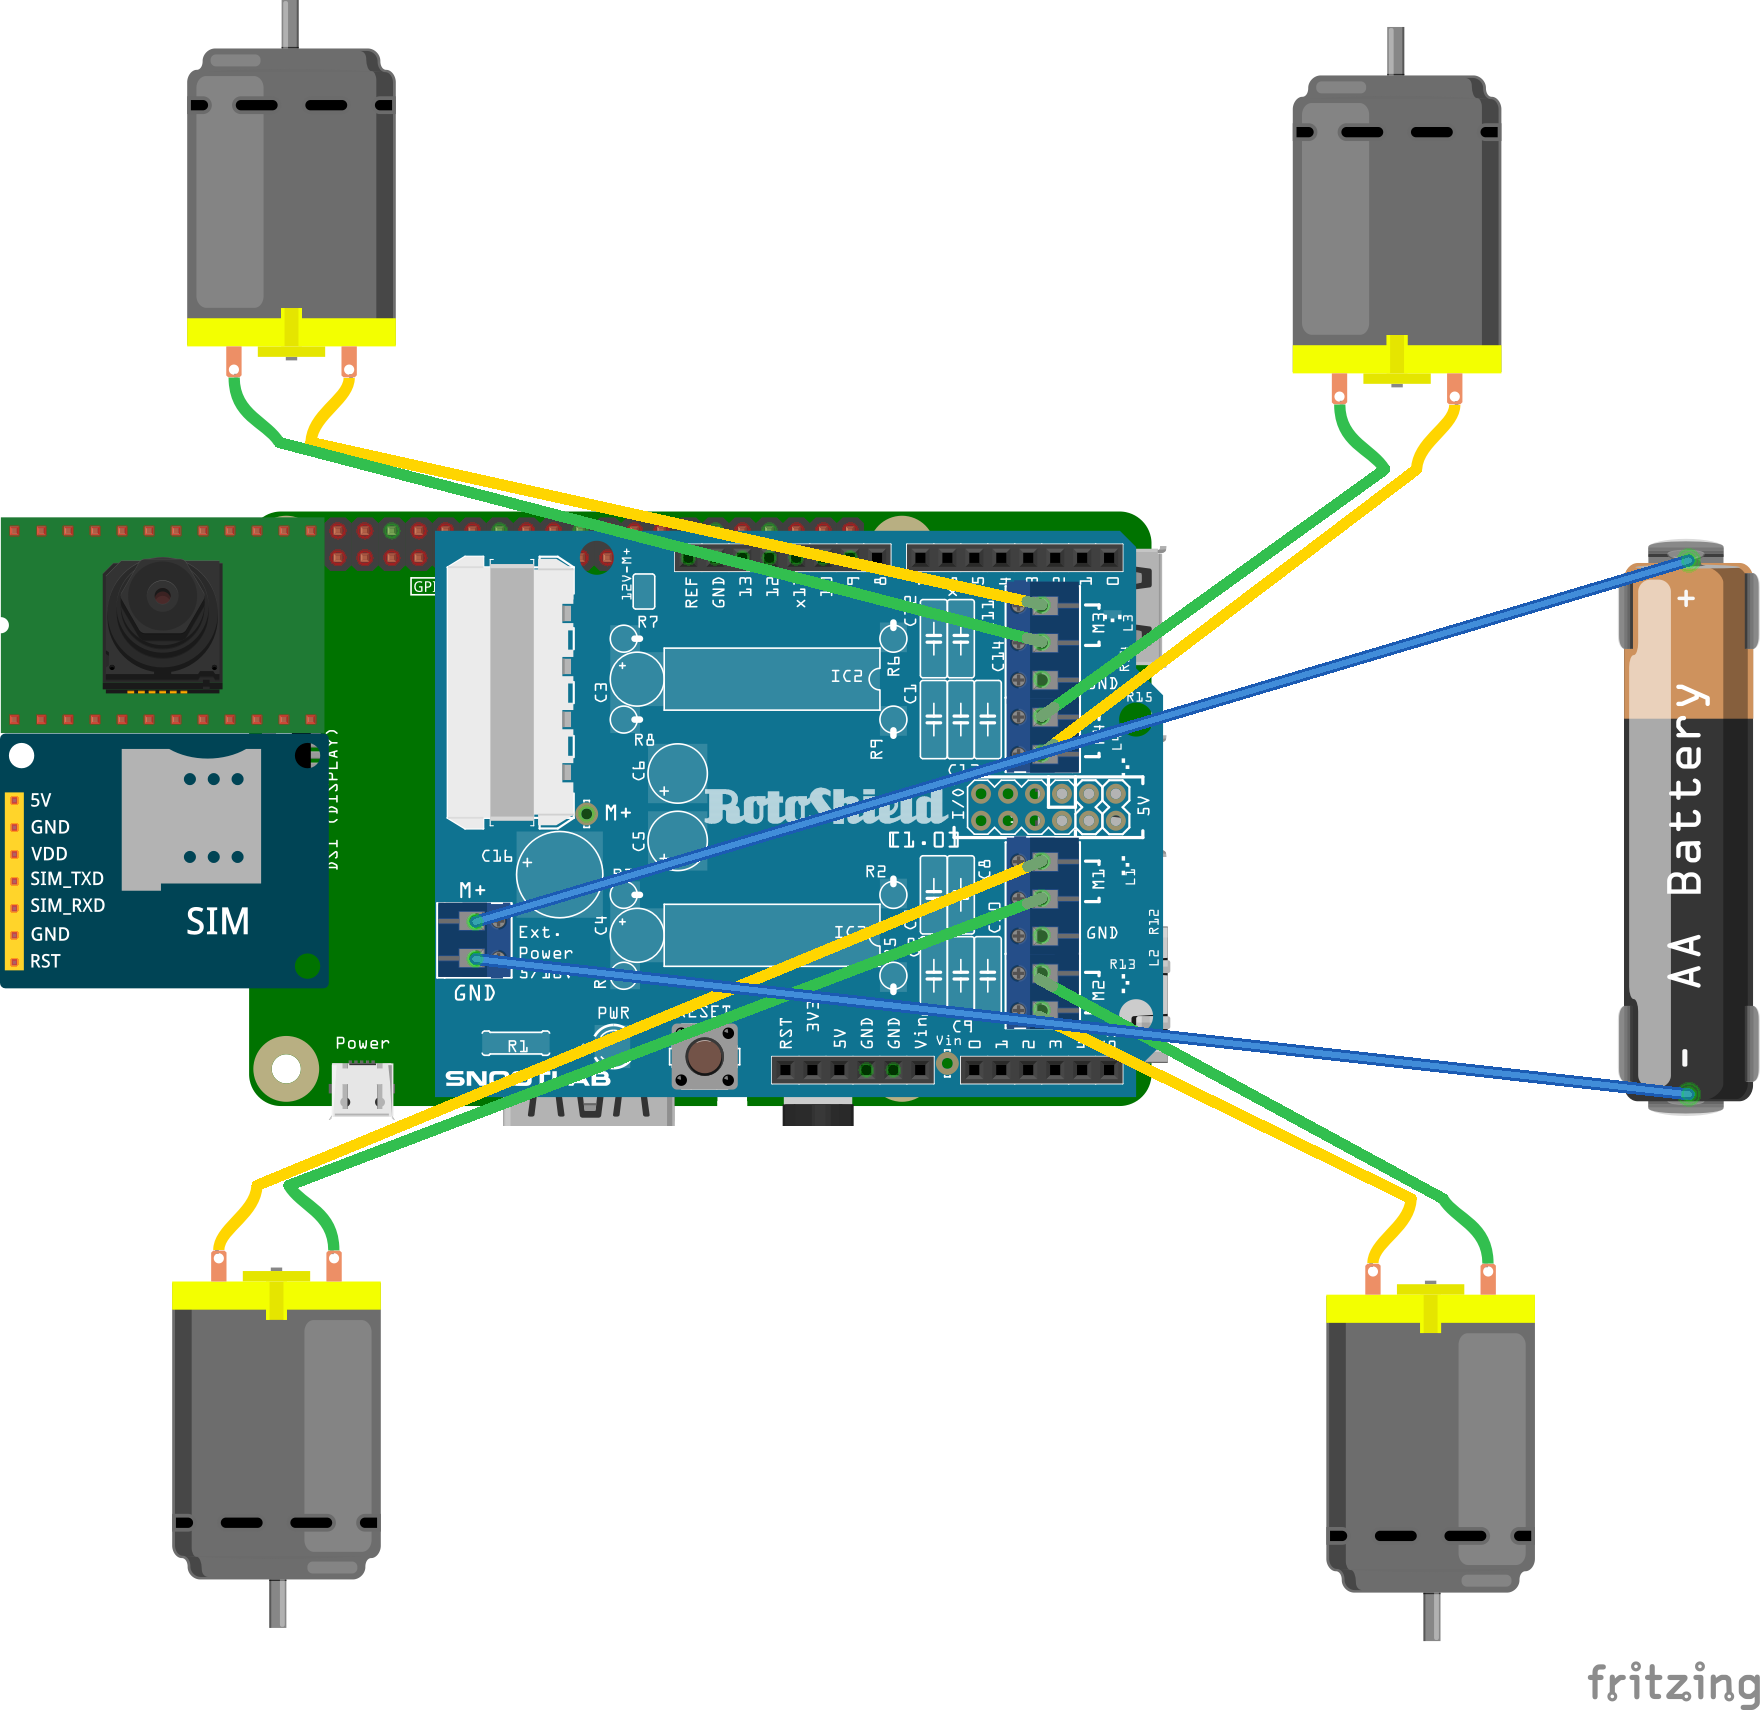
\includegraphics[keepaspectratio]{img/land-drone-bb.png}
    \caption{Robot Scheme}
\end{figure}

The software components running on the robot are the engine control and the \
I/O control (handling all outside communication and the camera itself for \
performance reasons).
In order to enforce low couping between these components and other components \
that could be added in the future, they are deployed separately and run in \
different processes.
The only means of communication is a queue, more specifically a RabbitMQ that \
runs on the robot.
The queue is used in order to transmit commands from the I/O control to the \
engine control for now.
This decoupled architecture prevents changes in a component from affecting \
other components and allows independently deploying several components, thus \
increasing extendability.


\subsection{Image transmission}
\label{subsec:analysis-image-transmission}
 I needed to devise an algorithm that would allow to one source to send images to several receivers that are
 not on the same network and at considerable distances, and at the same time having a delay as small as possible.
 Since the sender and the receivers won't be on the same network, they will need to interact via a 3rd component,
 a server that runs in cloud.

 The image needs to go through 2 different paths in order to get from the robot to the \
user that controls it. \
The first path is from robot to the cloud server that acts as a proxy. \
Since this communication is initiated by the client, the UDP protocol, which is faster than \
TCP, can be used. \
However, UDP packets have a small upper size limit (~500 bytes), which if surpassed, may cause \
the packet to be dropped on the way. \
For this reason, each image needs to be split into several smaller packets that can be safely \
transmitted over UDP. \
Since the protocol does not guarantee the order in which packets arrive at the destination, \
each one must contain 2 identifiers: one that uniquely identifies each image, and one that \
uniquely identifies the order of the packet in its image. \
Using these 2, the image can be safely reconstructed from the UDP packets. \
While the second identifier (for packets in an image) can be simply an index, the first \
identifier (for images) was chosen to be the unix timestamp in milliseconds at which the \
image was taken.

The second path that the image needs to go through is from the proxy server to \
multiple (web) clients connected to that server.
As mentioned above, this path should be using TCP sockets.
The best way to send data in a continuous stream from server to multiple web \
clients is using web sockets, which are supported by all modern browsers.

\begin{figure}[ht]
    \label{fig:video-flow}
    %\centering
    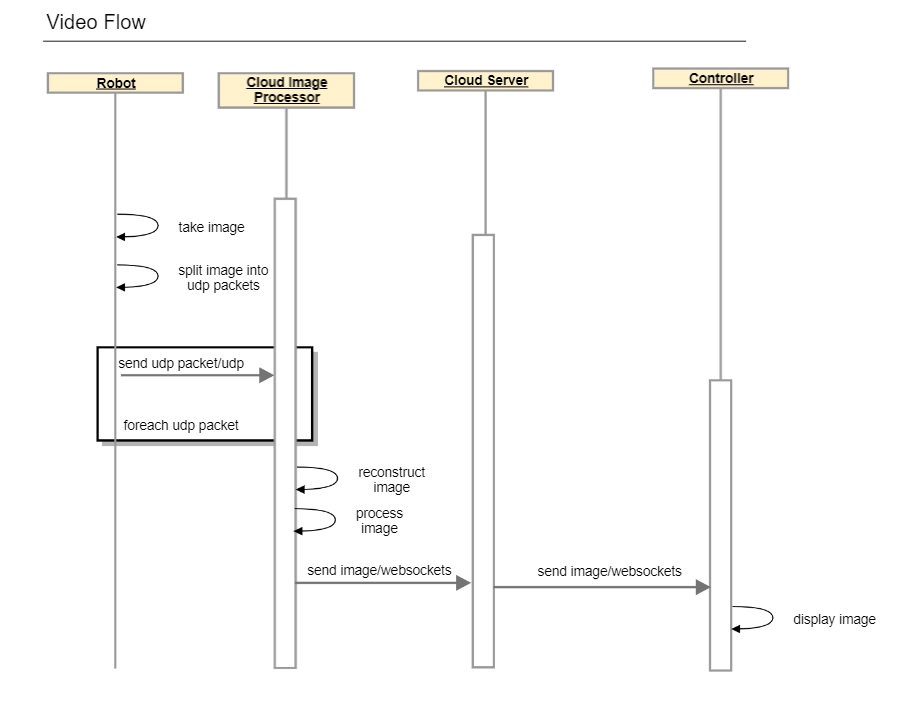
\includegraphics[width=15cm, height=20cm,keepaspectratio]{img/video-flow.png}
    \caption{Video Flow}
\end{figure}

As for the commands sent from the controller ot the drone, there are two possible \
options: using websockets or using a REST API.
In this case, the websockets present an advantage caused by the fact that they \
use an already existing connection, as opposed to using a REST API, which would \
require a new separate connection for each command to be sent.

\begin{figure}[ht]
    \label{fig:command-flow}
    %\centering
    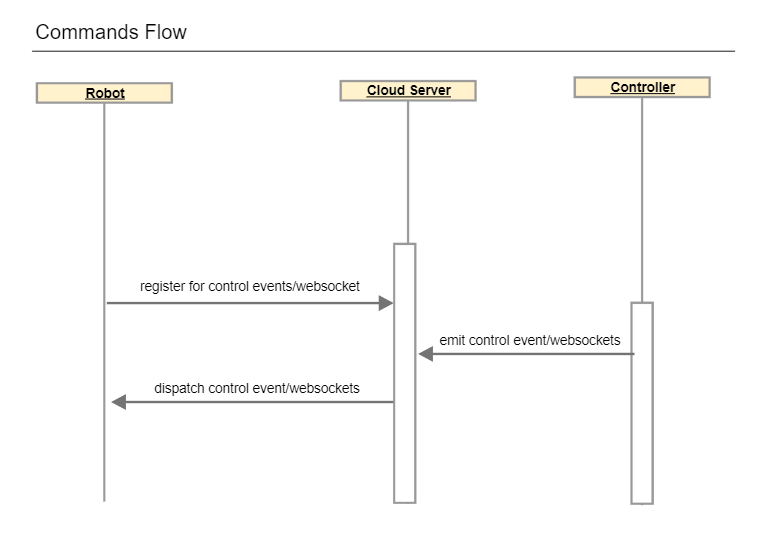
\includegraphics[width=15cm, height=20cm,keepaspectratio]{img/command-flow.png}
    \caption{Command Flow}
\end{figure}


%\chapter{Detailed Design and Implementation}
\label{ch:implementation}

% todo: detaliere fiecare chema

% results: rezultate intermediare, rezultate finale (hardware timp de raspuns, timp duratie transmitere, timp procesare imagine, tabele acuracy, procentaj detectie fete, procentaj recunoastere fete)
% pe cd: cod + documentatie
% gdpr compliance

\section{Introduction}
\label{sec:implementation-introduction}
This project contains 4 different components that are deployed in different \
places:
\begin{enumerate}
    \item the robot application (deployed and running on the actual robot)
    \item the proxy server that acts as an intermediary between the user \
            controlling the robot and the robot; \
            it runs in a kubernetes \
            cluster in the cloud (GKE, more precisely)
    \item an angular web application that is used to control the robot; \
            it is \
            deployed in the same cloud as the proxy server, but runs in the \
            user's browser
    \item the algorithm used to split an image into several UDP-ready packets \
            and to reconstruct the image from said packets; \
            the algorithm is published as a public package that is imported by \
            both the robot application and the web application
\end{enumerate}

Each component's detailed design and implementation will be detailed below.

\section{Robot Application}
\label{sec:robot-application}
I have chosen to run the robot application on a Raspberry PI 3 both \
because of the support for high-level development languages (Python, \
NodeJS, as opposed to VHDL/Verilog), and because of the support for \
third party modules/application (in this instance, RabbitMQ).

Physically, the robot consists of a platform with 4 wheels, a Raspberry PI, \
batteries and a camera, all connected with wires.

From a software point of view, it consists of 2 independent modules communicating \
with one another via RabbitMQ queues. \
The modules are engine control and external comms. \
The engine control module controls the 4 wheels independently and can make the \
robot go forward, reverse and steer. \
The external comms has 2 roles: capture video from camera to transmit it to the \
server, and listen for commands from the remote server in order to transmit them \
to the engine control via RabbitMQ.

Having separate processes leads to low couping and ensures that changes in one \
component do not affect other components.

%Together with the previous chapter takes about 60\% of the paper.
%
%The purpose of this chapter is to document the developed application such a way that it can be maintained and \
%developed later. \
%A reader should be able (from what you have written here) to identify the main functions of the application.
%
%The chapter should contain (but not limited to):
%\begin{itemize}
%    \item a general application sketch/scheme,
%    \item a description of every component implemented, at module level,
%    \item class diagrams, important classes and methods from key classes.
%\end{itemize}


%\chapter{Testing and Validation}

About 5\% of the paper
\section{Title}
\section{Other title}

\chapter{User's manual}

%\section{Hardware}
%In order to run the application, an administrator requires at leat a \
%physical or virtual machine with a x64 processor, 2 GB RAM and 50GB hard disk.\
%Ideally, the machine should be running a Linux OS, but Windows is also supported.
%
%\section{Software Dependencies}
%In the following section, we will present the installation steps on Debian-based OS \
%(Debian, Ubuntu, Mint).
%
%There are 3 main dependencies: Apache Tomcat(the environment used to run the \
%application server), MySQL(used to host the application database) and NginX (web \
%server which will be used as a reverse proxy and where we will setup the SSL encryption).\
%However, before installing any software the administrator must update the package \
%repositories by running the following command in a terminal:

%\begin{verbatim}
%sudo apt update
%\end{verbatim}
%
%\subsection{MySQL}
%In order to install MySQL server, you need to run the following commands:
%\begin{verbatim}
%apt install mysql-server
%/etc/init.d/mysql start
%\end{verbatim}
%
%Then, you need to add a custom admin user:
%\begin{verbatim}
%mysql -u root -p
%mysql>CREATE USER 'user'@'%' IDENTIFIED BY 'password';
%mysql>GRANT ALL PRIVILEGES ON *.* TO 'user'@'%' WITH GRANT OPTION;
%mysql>FLUSH PRIVILEGES;
%mysql>quit;
%\end{verbatim}
%Then, you need to edit the \textit{my.cnf} file to allow remote connections to the \
%mysql server. Usually it is located at \textit{/etc/mysql/my.cnf}, but this may change \
%depending on the OS. You need to change the \textit{bind-address} option as below:
%\begin{verbatim}
%bind-address = 0.0.0.0
%\end{verbatim}
%
%Then restart the mysql service with the command \textit{sudo /etc/init.d/mysql restart}.
%
%
%\subsection{Apache Tomcat}
%
%In order to install Apache Tomcat, a user first needs to install Java on the system. \
%This can be done by running the following command (This will install both the runtime \
%environment and the development kit.):
%
%\begin{verbatim}
%sudo apt install default-jdk
%\end{verbatim}
%
%In order to validate the installation, run the following commands:
%\begin{verbatim}
%java -version
%javac -version
%\end{verbatim}
%If no error is presented, the the java environment was installed successfully.
%
%Next, you need to add a \textit{tomcat} user and user group. The home directory will \
%be \textit{/opt/tomcat}, and the shell \textit{/bin/false}, so that no user can login \
%as tomcat.
%
%\begin{verbatim}
%sudo groupadd tomcat
%sudo mkdir -p /opt/tomcat
%sudo useradd -s /bin/false -g tomcat -d /opt/tomcat tomcat
%\end{verbatim}
%
%Next, you need to install additional dependencies:
%\begin{verbatim}
%sudo apt install curl
%\end{verbatim}
%Then, download the tomcat sources and extract them:
%\begin{verbatim}
%cd /tmp
%curl -O apache.mirrors.ionfish.org/tomcat/tomcat-9/v9.0.10/src/apache-tomcat-9.0.10-src.tar.gz
%tar xzvf apache-tomcat-9.0.10-src.tar.gz -C /opt/tomcat --strip-components=1
%\end{verbatim}
%
%Next, you need to update user permissions:
%\begin{verbatim}
%cd /opt/tomcat
%sudo chgrp -R tomcat /opt/tomcat
%sudo chmod -R g+r conf
%sudo chmod g+x conf
%sudo chown -R tomcat webapps/ work/ temp/ logs/
%\end{verbatim}
%
%Next, you need to create the service file. For that, you need the \
%\textit{JAVA\_HOME}. In order to obtain it, run the command: \
%\textit{sudo update-java-alternatives -l}. The output should be \
%something similar to below:
%\begin{verbatim}
%java-1.8.0-openjdk-amd64       1081       /usr/lib/jvm/java-1.8.0-openjdk-amd64
%\end{verbatim}
%
%The \textit{JAVA\_HOME} can be constructed by appending \textit{/jre} \
%to the last column. Now you can create the file \
%\textit{/etc/systemd/system/tomcat.service} and put the following \
%contents in it:
%
%\begin{verbatim}
%[Unit]
%Description=Apache Tomcat Web Application Container
%After=network.target
%
%[Service]
%Type=forking
%
%Environment=JAVA_HOME=/usr/lib/jvm/java-1.8.0-openjdk-amd64/jre
%Environment=CATALINA_PID=/opt/tomcat/temp/tomcat.pid
%Environment=CATALINA_HOME=/opt/tomcat
%Environment=CATALINA_BASE=/opt/tomcat
%Environment='CATALINA_OPTS=-Xms512M -Xmx1024M -server -XX:+UseParallelGC'
%Environment='JAVA_OPTS=-Djava.awt.headless=true -Djava.security.egd=file:/dev/./urandom'
%
%ExecStart=/opt/tomcat/bin/startup.sh
%ExecStop=/opt/tomcat/bin/shutdown.sh
%
%User=tomcat
%Group=tomcat
%UMask=0007
%RestartSec=10
%Restart=always
%
%[Install]
%WantedBy=multi-user.target
%\end{verbatim}
%
%Next, you need to reload the systemd daemon in order for it to discover \
%the new tomcat service, and then you can start the service.
%\begin{verbatim}
%sudo systemctl daemon-reload
%sudo systemctl start tomcat
%\end{verbatim}
%In the installation description section your should detail the hardware \
%and software resources needed for installing and running the application, \
%and a step by step description of how your application can be \
%deployed/installed. An administrator should be able to perform the \
%installation/deployment based on your instructions.
%
%In the user manual section you describe how to use the application from \
%the point of view of a user with no inside technical information; this \
%should be done with screen shots and a stepwize explanation of the interaction. \
%Based on user's manual, a person should be able to use your product.

\chapter{Conclusions}

About. 5\% of the whole

Here your write:
\begin{itemize}
\item a summary of your contributions/achievements,
\item a critical analysis of the achieved results,
\item a description of the possibilities of improving/further development.
\end{itemize}
\section{Title}
\section{Other title}


%\addcontentsline {toc}{chapter}{Bibliography}
\bibliographystyle{IEEEtran} 
\bibliography{thesis}%same file name as for .bib


\appendix
\chapter{Relevant code}

\begin{verbatim}
 /** Maps are easy to use in Scala. */
object Maps {
  val colors = Map("red" -> 0xFF0000,
                   "turquoise" -> 0x00FFFF,
                   "black" -> 0x000000,
                   "orange" -> 0xFF8040,
                   "brown" -> 0x804000)
  def main(args: Array[String]) {
    for (name <- args) println(
      colors.get(name) match {
        case Some(code) =>
          name + " has code: " + code
        case None =>
          "Unknown color: " + name
      }
    )
  }
}
\end{verbatim}

\chapter{Other relevant information (demonstrations, etc.)}


\chapter{Published papers}

\end{document}

\begin{document}



\end{document}
\begin{document}



\end{document}
\begin{document}



\end{document}

% todo: https://bford.info/pub/net/p2pnat/ nat hole pucnhing
